\documentclass[12pt]{article}
% Para submissão: troque sbc-like por sbc-template (ver comentário em sbc-like.sty).
\usepackage{sbc-like}
\usepackage[utf8]{inputenc}
\usepackage[T1]{fontenc}
\usepackage[brazilian]{babel}
\usepackage{graphicx}
\usepackage{booktabs}
\usepackage{xcolor}
\usepackage{tikz}
\usetikzlibrary{arrows.meta,positioning,calc}
\usepackage{caption}
\usepackage{amsmath}
\usepackage[hidelinks]{hyperref}
\usepackage{url}
\captionsetup{font=small,labelfont=bf}

% Marcador de conteúdo que depende de execução ainda não realizada.
\newcommand{\pendente}[1]{{\color{red}\textbf{[PENDENTE: #1]}}}

\begin{document}

\sbctitle{Malha de \textit{Continuous Evals} Guiada por Mutação\\ para Geração de Testes com LLM}

\begin{center}
\textbf{Andriano Toazza, Gabriel Vanz}\\[2pt]
Programa de Pós-Graduação em Computação Aplicada (PPGCA)\\
\texttt{\{andriano.toazza, gabriel.vanz\}@\pendente{domínio institucional}}
\end{center}

\begin{abstract}
Cobertura de linha é uma métrica fraca de qualidade de testes, e testes gerados por modelos de linguagem (LLMs)
tendem a cobrir código sem detectar defeitos. Este trabalho, do estágio \textit{Test} do SDLC AI-Native, propõe e
implementa uma malha de \textit{continuous evals} em que um agente de LLM gera testes unitários em Vitest para módulos
de bibliotecas TypeScript reais, o Stryker mede o \textit{mutation score} e os mutantes sobreviventes realimentam o
agente em um laço executado no GitHub Actions. O desenho compara cinco condições (testes humanos, \textit{zero-shot},
convenções de projeto, amostragem independente com o mesmo orçamento e laço com feedback), usa um \textit{split} de
mutantes para separar o sinal de feedback do sinal de avaliação e define guardrails contra testes triviais. Apresentamos
o arcabouço (código aberto, com testes unitários e validação de ponta a ponta), o protocolo estatístico, o
\textit{baseline} humano medido em 9 módulos de 4 bibliotecas e a primeira execução das quatro condições com LLM
(\texttt{gemini-3.5-flash-lite}, 3 repetições por módulo). A condição com laço de feedback (C3) teve a maior mediana de
\textit{mutation score} no grupo de avaliação (80,3\%, contra 70,0\% em C1, 76,1\% em C2 e 79,0\% em C2r). Porém, com o
orçamento igualado, a vantagem sobre C2r (4,0 pontos percentuais) não se distingue de zero (Wilcoxon pareado unilateral,
$p$ ajustado $=0{,}109$, $n=8$ módulos), de modo que H1 \textbf{não é sustentada}; só a comparação com C2 é
significativa ($p$ ajustado $=0{,}047$, $n=6$). A cobertura de linha chega a 100\% em todas as condições com LLM, e a taxa de
\textit{runs} com ao menos um teste válido varia de 63,0\% (C2) a 88,9\% (C2r). Com 9 módulos, os resultados têm baixo poder
e devem ser lidos como exploratórios.
\end{abstract}

{\renewcommand{\abstractname}{Abstract}\begin{abstract}
\noindent Line coverage is a weak proxy for test quality, and LLM-generated tests often cover code
without detecting faults. We present a mutation-guided continuous-evals loop for LLM test generation: an agent writes
Vitest tests for real TypeScript libraries, Stryker computes the mutation score, and surviving mutants are fed back to
the agent in a GitHub Actions pipeline. The design compares five conditions (human tests, zero-shot, project
conventions, equal-budget independent sampling, and feedback loop), uses a mutant hold-out split and guardrails against
trivial tests. We release the framework, the statistical protocol, a measured human baseline over 9 modules from 4
libraries, and a first run of the four LLM conditions (\texttt{gemini-3.5-flash-lite}, 3 repetitions per module). The
feedback loop (C3) had the highest median mutation score on the held-out mutants (80.3\%, versus 70.0\% for C1, 76.1\% for
C2 and 79.0\% for C2r). With equal budget, however, the advantage over C2r (4.0 percentage points) is not distinguishable
from zero (one-sided paired Wilcoxon, adjusted $p=0.109$, $n=8$ modules), so H1 is \textbf{not supported}; only the
comparison with C2 is significant (adjusted $p=0.047$, $n=6$). Line coverage reaches 100\% in every LLM condition, and the
share of runs with at least one valid test ranges from 63.0\% (C2) to 88.9\% (C2r). With 9 modules the results have low
power and should be read as exploratory.
\end{abstract}}

\section{Introdução}

A adoção de IA generativa no desenvolvimento de software passou da aceleração da escrita de código para a
reorganização do ciclo de vida inteiro. No paradigma AI-Native SDLC adotado na disciplina, o estágio de testes deixa
de ser um portão rígido no fim do desenvolvimento e passa a ser uma malha de avaliação contínua (\textit{continuous
evals}) integrada ao fluxo de implementação e ao CI. Em paralelo, o conhecimento do projeto é codificado em arquivos
legíveis por humanos e executáveis por máquinas, como o \texttt{CLAUDE.md}.

Nesse contexto, LLMs são usados para gerar testes unitários, mas a pergunta relevante não é se os testes gerados
compilam, passam ou cobrem linhas, e sim se eles \textbf{detectam defeitos}. A cobertura mede o que foi executado, não o que
foi verificado \cite{inozemtseva2014}. O teste de mutação mede diretamente a capacidade de detecção: introduz pequenas
alterações sintáticas (mutantes) no código e verifica se os testes falham \cite{jia2011,papadakis2019}. Mutantes que
sobrevivem apontam lacunas concretas, e isso os torna um sinal natural de feedback para um agente.

Este trabalho investiga a seguinte \textbf{pergunta de pesquisa}: \emph{o feedback de mutantes sobreviventes aumenta o
mutation score de testes gerados por LLM, e a que custo, comparado a testes escritos por humanos?} Formulamos três
hipóteses:
\begin{itemize}
  \item \textbf{H1.} Testes gerados com o laço de mutantes (C3) têm \textit{mutation score} maior que \textit{zero-shot}
  (C1), que o uso de convenções de projeto (C2) e que a amostragem independente com o mesmo orçamento (C2r).
  \item \textbf{H2.} A cobertura de linha sobe sem que o \textit{mutation score} suba na mesma proporção: cobrir não é
  detectar.
  \item \textbf{H3.} O ganho de C3 tem retorno decrescente após poucas iterações, com custo em tokens por ponto de
  \textit{score} crescente.
\end{itemize}

\noindent\textbf{Contribuições.} (i) Um arcabouço aberto e testado que implementa o laço, os guardrails e o registro de
métricas por iteração; (ii) um desenho experimental com controle de orçamento (C2r) e \textit{hold-out} de mutantes, que
evita que o agente seja avaliado no mesmo sinal que otimiza; (iii) o \textit{baseline} humano medido em 9 módulos reais,
com achados de engenharia sobre a medição; (iv) o protocolo estatístico para H1--H3; e (v) a primeira execução das
quatro condições com LLM, com resultados que não sustentam H1 quando o orçamento é igualado (Seção~\ref{sec:resultados}).

\section{Fundamentação e trabalhos relacionados}

\textbf{Teste de mutação.} Mutantes são programas ligeiramente alterados por operadores como troca de operador
aritmético ou relacional, remoção de condicionais e alteração de literais. Um mutante é \emph{morto} se algum teste falha
sobre ele e \emph{sobrevive} caso contrário \cite{demillo1978}. O \textit{mutation score} é a razão entre mutantes
detectados e mutantes válidos. Usamos o critério do Stryker: $\text{MS}=\frac{K+T}{K+T+S+N}$, em que $K$ são mortos, $T$
\textit{timeouts}, $S$ sobreviventes e $N$ mutantes sem cobertura; erros de compilação, de execução e mutantes ignorados
saem do denominador. Mutantes equivalentes, que não alteram o comportamento, não podem ser mortos e fazem o \textit{score}
subestimar a qualidade; tratamos isso como limitação e como análise de sensibilidade (Seção~\ref{sec:ameacas}). Há
evidência de que mutantes são um substituto razoável para defeitos reais \cite{just2014} e de que o uso de teste de
mutação em desenvolvimento muda práticas de teste \cite{petrovic2021}.

\textbf{Cobertura versus eficácia.} Inozemtseva e Holmes \cite{inozemtseva2014} mostram que a correlação entre
cobertura e eficácia de suítes é fraca quando se controla o tamanho da suíte. Essa é a base conceitual de H2.

\textbf{Geração de testes com LLM.} Schäfer et al.\ \cite{schafer2024} avaliaram a geração de testes unitários por LLM
para pacotes JavaScript com refinamento iterativo de testes que falham, reportando cobertura mediana da ordem de 70\%.
Alshahwan et al.\ \cite{alshahwan2024} descrevem, na Meta, filtros em camadas (compila, passa, aumenta cobertura) sobre
testes melhorados por LLM. Dakhel et al.\ \cite{dakhel2024} propõem usar mutantes sobreviventes para refinar o prompt
(MuTAP), avaliando em programas Python, e Foster et al.\ \cite{foster2025} descrevem geração de testes guiada por
mutantes em escala industrial. Até onde conseguimos verificar sem acesso a busca bibliográfica, nosso desenho se
diferencia por (i) isolar o efeito do \emph{feedback} do efeito de \emph{mais tentativas} com C2r, (ii) separar mutantes de
feedback e de avaliação, (iii) comparar com a suíte humana do próprio projeto sob o mesmo escopo de mutação, (iv) reportar
curvas de custo por iteração e (v) estratificar por risco de memorização. Uma revisão sistemática completa é trabalho futuro.

\textbf{AI-Native SDLC.} No estágio \textit{Test}, a abordagem tradicional concentra portões de QA no fim das fases; a
abordagem AI-Native integra malhas de avaliação contínua ao fluxo de implementação e ao CI. Nossa malha instancia essa
ideia: cada alteração gera testes, mede-os com um oráculo automático (mutantes) e decide se continua iterando.

\section{Metodologia}

\subsection{Arquitetura}

A Figura~\ref{fig:arq} resume o pipeline, implementado em TypeScript e executado em uma matriz do GitHub Actions
(módulo $\times$ condição $\times$ repetição). Para cada \textit{run}, o agente monta o prompt, chama o LLM, extrai o arquivo
de teste, aplica guardrails estáticos, executa o Vitest sobre o código original (com até 2 reparos) e então mede a
cobertura (provedor v8), a estabilidade (3 reexecuções) e o \textit{mutation score} (Stryker com análise de cobertura por
teste). Em C3, os sobreviventes do grupo de feedback voltam ao prompt até o critério de parada.

\begin{figure}[t]
\centering
\begin{tikzpicture}[
  box/.style={draw,rounded corners=2pt,minimum height=9mm,minimum width=24mm,align=center,font=\footnotesize,inner sep=3pt},
  arr/.style={-{Stealth[length=2mm]},thick}]
  \node[box] (src) at (0,0) {Código-fonte\\do módulo};
  \node[box,fill=blue!8] (llm) at (3.2,0) {Agente\\LLM};
  \node[box] (guard) at (6.4,0) {Guardrails\\+ Vitest};
  \node[box] (str) at (9.6,0) {Stryker\\+ \textit{split}};
  \node[box] (stop) at (9.6,-1.9) {Parar?\\{\scriptsize $k{=}N$ ou sem sobreviventes}};
  \node[box] (rep) at (9.6,-3.7) {Relatório\\{\scriptsize \textit{score} e custo}};
  \draw[arr] (src)--(llm); \draw[arr] (llm)--(guard); \draw[arr] (guard)--(str);
  \draw[arr] (str)--(stop);
  \draw[arr] (stop)--node[right,font=\scriptsize]{sim}(rep);
  \draw[arr] (stop.west) -- node[above,font=\scriptsize]{não: sobreviventes do grupo \textit{feedback}} (llm |- stop.west) -- (llm.south);
\end{tikzpicture}
\caption{Malha de \textit{continuous evals}: mutantes sobreviventes do grupo de feedback realimentam o agente.}
\label{fig:arq}
\end{figure}

\subsection{Sujeitos e seleção de módulos}

Usamos bibliotecas pequenas, em TypeScript, com suíte humana em Vitest, licença MIT e funções puras (sem rede, banco ou
I/O): \texttt{ufo}, \texttt{defu}, \texttt{pathe} e \texttt{knitwork}, cada uma fixada em um \textit{commit}. A unidade de
análise é o \textbf{módulo} (um arquivo \texttt{.ts}), pareado entre condições, porque quatro bibliotecas seriam
poucas observações. Consideramos 17 módulos candidatos e medimos 14 com a suíte humana e o Stryker (\texttt{scule} e \texttt{ohash} não puderam ser medidos por falhas de ferramenta, e \texttt{pathe/\_glob} ficou de fora por tempo); aplicamos, \textbf{antes} de qualquer
execução de LLM, os critérios: pelo menos 50 mutantes válidos (para que cada metade do \textit{split} tenha $\geq 25$) e
\textit{score} humano de no máximo 92\% (para haver espaço de melhoria). Restaram 9 módulos (Tabela~\ref{tab:sujeitos}).
O \texttt{scule} usa Vitest 1.x, incompatível com o executor do Stryker usado.

\begin{table}[t]
\centering\small
\begin{tabular}{llrrr}
\toprule
Biblioteca & Módulo & LOC & Mutantes válidos & MS suíte humana (\%) \\
\midrule
ufo & query & 138 & 78 & 85.9 \\
ufo & parse & 229 & 150 & 86.0 \\
ufo & punycode & 100 & 180 & 73.9 \\
ufo & url & 148 & 90 & 75.6 \\
ufo & utils & 775 & 470 & 84.5 \\
defu & defu & 71 & 67 & 79.1 \\
pathe & \_path & 314 & 397 & 89.7 \\
pathe & utils & 134 & 87 & 80.5 \\
knitwork & string & 104 & 70 & 31.9 \\
\bottomrule
\end{tabular}

\caption{Módulos incluídos. ``Mutantes válidos'' exclui erros de compilação/execução. MS: \textit{mutation score} da
suíte humana completa do repositório, medido no commit fixado.}
\label{tab:sujeitos}
\end{table}

\subsection{Condições}

Todas usam o mesmo modelo e parâmetros. \textbf{C0}: testes humanos do módulo (e, como referência superior,
\textbf{C0-suite}: toda a suíte humana, com a mutação restrita ao módulo). \textbf{C1}: \textit{zero-shot}, apenas o
código-fonte. \textbf{C2}: C1 mais um arquivo de convenções (estilo, estrutura, casos a cobrir), injetado no prompt;
o arquivo é deliberadamente livre de menções a teste de mutação para não contaminar o efeito de C3. \textbf{C2r}:
$1+N$ amostras independentes de C2, escolhendo-se a de maior \textit{score} no grupo de feedback; é o controle de
orçamento. \textbf{C3}: C2 mais até $N=5$ iterações com até 20 sobreviventes do grupo de feedback, cada um com linha,
operador, trecho original e trecho mutado. A iteração seguinte parte da melhor iteração válida até o momento.

\subsection{\textit{Split} de mutantes e guardrails}

Como C3 otimiza o mesmo \textit{score} usado para avaliá-lo, dividimos os mutantes de cada módulo em dois grupos
determinísticos e estratificados por operador: dentro de cada operador, ordenam-se os mutantes por
$\text{SHA-256}(\text{seed}\,\|\,\text{chave})$ e alternam-se os grupos \textit{feedback} e \textit{avaliação}. O grupo
é calculado sobre todos os mutantes gerados, independentemente do estado, e portanto é idêntico em todas as condições. Só
sobreviventes de \textit{feedback} chegam ao agente; a métrica principal de H1 é o \textit{score} no grupo de avaliação.
Os guardrails rejeitam: alteração do código-fonte; \texttt{.skip/.only/.todo}; \texttt{expect(true)} e tautologias;
testes sem \textit{assertion}; imports além do Vitest e do módulo; rede, relógio e aleatoriedade sem controle; e
testes que falham em reexecução (marcados como instáveis).

\subsection{Métricas e análise estatística}

Por \textit{run} e por iteração registramos \textit{mutation score} (avaliação, feedback e total), cobertura de linha e de ramo,
tokens de entrada e saída (os reportados pela API, incluindo reparos), custo de referência em USD, tempo, iterações,
taxa de iterações válidas, estabilidade e tamanho da suíte. A unidade estatística é o módulo (mediana das repetições).
Para H1 usamos Wilcoxon pareado unilateral com correção de Holm, tamanho de efeito (Cliff $\delta$) e IC bootstrap de
95\%; para H2, a diferença entre o ganho de cobertura e o de \textit{score} (Wilcoxon e Spearman) e a lacuna
$\text{cob}_{\text{linha}}-\text{MS}$; para H3, as curvas por iteração, o teste de Friedman sobre os ganhos marginais, o teste de
tendência de Page e os tokens por ponto percentual. O \textit{score} é também reportado sobre o conjunto de mutantes
mortos por qualquer condição ($\text{MS}_{\text{killable}}$), um limite inferior prático para o teto atingível dado que
equivalência é indecidível.

Como a análise principal só considera \textit{runs} em que o modelo produziu ao menos um teste válido, reportamos
também a taxa de validade por condição (de \textit{runs} e de iterações), contando apenas desfechos atribuíveis ao modelo:
falhas de infraestrutura, como limite de cota da API ou \textit{timeout}, são refeitas e não entram nos denominadores.
Para expor o viés de sobrevivência, repetimos as comparações de H1 em uma análise de sensibilidade exploratória, definida
depois de observadas as primeiras execuções e, portanto, não prevista no protocolo original, em que um \textit{run} sem
nenhum teste válido conta como \textit{score} zero.

Três \textit{runs} de \texttt{pathe/path} além das três repetições previstas (C1 nas repetições 4 e 8, e C2 na 7) foram
coletados em um lote anterior e excluídos da análise, para não dar a esse módulo mais repetições que aos demais; o
desvio está registrado na seção 12 do protocolo.

\subsection{Modelo, reprodutibilidade e uso de IA}

O modelo é acessado por API de camada gratuita (Google AI Studio), com ID exato registrado em cada \textit{run}
(\texttt{gemini-3.5-flash-lite}, coleta de 22 a 26 de novembro de 2026), $T=0{,}7$ em todas as condições e saída máxima de 8192 tokens. Como modelos
gratuitos mudam, arquivamos todos os prompts, respostas brutas e relatórios do Stryker. O custo real é zero; reportamos
um custo de referência com preços fixos para discussão. O código, o protocolo, os dados e a análise estão no repositório
\pendente{URL do repositório público}.

\textbf{Uso de IA no desenvolvimento do trabalho.} Utilizamos o Claude (Anthropic) para propor o desenho experimental,
escrever o código do arcabouço e dos scripts de análise, executar as medições de seleção e o \textit{baseline} C0 em ambiente
isolado e redigir o rascunho deste texto. O registro detalhado, incluindo erros do assistente que foram detectados e
corrigidos, está em \texttt{AI\_USAGE.md}. A IA não executou as condições com LLM: elas foram executadas pelos autores no
GitHub Actions, e os números reportados aqui vêm dos \texttt{result.json} resultantes, processados por
\texttt{analysis/analyze.py}. Os autores revisaram o
conteúdo \pendente{confirmar revisão integral pelos autores antes da entrega}.

\section{Resultados}
\label{sec:resultados}

\subsection{\textit{Baseline} humano (C0)}

A Tabela~\ref{tab:c0} mostra o \textit{baseline} humano medido pelo próprio pipeline, com os testes humanos mapeados a cada
módulo. O \textit{score} total mediano da suíte humana no escopo do módulo é 79,1\% (de 12,2\% a 89,7\%), com cobertura de linha mediana de 95,5\%. A lacuna mediana entre cobertura de linha e \textit{score} é de 19,5 pontos percentuais (de 8,5 a 56,6); isto é, mesmo testes humanos cobrem mais do que detectam, o que é coerente com a premissa de H2. O módulo com menor \textit{score} é \texttt{knitwork/string} (12,2\%). Ao usar toda a suíte do repositório (C0-suite), o \textit{score} mediano passa a 80,5\% (9 módulos pareados); a maior diferença entre escopos é de 28,0 pontos percentuais em \texttt{ufo/parse}. O escopo dos testes humanos, portanto, muda substancialmente o \textit{baseline}, e por isso ambos são reportados.


\begin{table}[t]
\centering\small
\begin{tabular}{llrrrr}
\toprule
Módulo & Mutantes & Cob. linha (\%) & Cob. ramo (\%) & MS\textsubscript{all} (\%) & MS\textsubscript{eval} (\%) \\
\midrule
defu/defu & 67 & 100.0 & 100.0 & 79.1 & 86.7 \\
knitwork/string & 81 & 68.8 & 71.4 & 12.2 & 11.4 \\
pathe/\_path & 397 & 99.3 & 98.4 & 89.7 & 89.2 \\
pathe/utils & 89 & 100.0 & 96.5 & 80.5 & 82.1 \\
ufo/parse & 150 & 71.0 & 52.8 & 58.0 & 57.7 \\
ufo/punycode & 180 & 95.2 & 75.8 & 73.9 & 78.4 \\
ufo/query & 78 & 96.4 & 96.0 & 85.9 & 88.9 \\
ufo/url & 90 & 95.5 & 62.9 & 75.6 & 76.7 \\
ufo/utils & 470 & 91.2 & 93.8 & 82.8 & 82.3 \\
\bottomrule
\end{tabular}

\caption{C0 (escopo módulo): suíte humana do módulo. MS\textsubscript{eval} e MS\textsubscript{all} no grupo de avaliação e no total.}
\label{tab:c0}
\end{table}

\subsection{Achados de engenharia da medição}

A execução do arcabouço sobre código real revelou problemas que afetariam a validade e que corrigimos antes da coleta:
(i) o Stryker exclui erros de execução (\textit{RuntimeError}) do denominador do \textit{score}, o que nosso protocolo
inicial não previa; (ii) a chave de identificação dos mutantes colidia para mutantes aninhados, que começam na mesma
posição e terminam em posições diferentes, o que corromperia o \textit{split}; (iii) com pnpm o plugin de Vitest do
Stryker precisa ser declarado explicitamente; (iv) Vitest 1.x é incompatível com o executor atual; (v) o escopo dos
testes humanos altera muito o \textit{baseline} (Seção anterior), por isso reportamos C0 em dois escopos; e (vi) vários
módulos têm poucos mutantes ou \textit{score} humano próximo de 100\%, o que cria efeito teto e motivou os critérios de
inclusão. Em um teste de fumaça com provedor simulado e testes escritos à mão, o executor completo (Vitest, cobertura,
Stryker, \textit{split} e esquema de resultado) funcionou de ponta a ponta; isso valida o encanamento e \textbf{não} é um
resultado experimental.

\subsection{Condições com LLM (C1, C2, C2r, C3)}

Executamos C1, C2, C2r e C3 com 3 repetições por módulo (111 \textit{runs} coletados; 108 previstos mais 3 excluídos, ver
a seção de Metodologia). As Tabelas~\ref{tab:cond} e~\ref{tab:h1} são geradas automaticamente por
\texttt{analysis/analyze.py} a partir dos \texttt{result.json}. Como os \textit{runs} sem teste válido saem da análise
principal, o número de módulos pareados em cada comparação é menor que 9, e os resultados abaixo devem ser lidos como
exploratórios.

\begin{table}[t]
\centering\small
\begin{tabular}{lrrrrrr}
\toprule
Cond. & $n$ & MS\textsubscript{eval} & MS\textsubscript{all} & Cob. linha & Tokens & US\$ ref. \\
\midrule
C0 & 9 & 82.1 & 79.1 & 95.5 & 0 & 0.0000 \\
C0-suite & 9 & 84.0 & 80.5 & 99.3 & 0 & 0.0000 \\
C1 & 0 & n/d & n/d & n/d & n/d & n/d \\
C2 & 0 & n/d & n/d & n/d & n/d & n/d \\
C2r & 0 & n/d & n/d & n/d & n/d & n/d \\
C3 & 0 & n/d & n/d & n/d & n/d & n/d \\
\bottomrule
\end{tabular}

\caption{Resumo por condição (medianas das execuções válidas). $n$: \textit{runs} usados; tokens e custo de referência acumulados
até a iteração selecionada, incluindo reparos.}
\label{tab:cond}
\end{table}

\begin{table}[t]
\centering\small
\begin{tabular}{lrrrrrr}
\toprule
Comparação & $n$ & $\Delta$ mediana & IC 95\% & Cliff $\delta$ & $p$ & $p_{Holm}$ \\
\midrule
C3 $>$ C1 & 0 & n/d & n/d & n/d & n/d & n/d \\
C3 $>$ C2 & 0 & n/d & n/d & n/d & n/d & n/d \\
C3 $>$ C2r & 0 & n/d & n/d & n/d & n/d & n/d \\
\bottomrule
\end{tabular}

\caption{H1: comparações pareadas por módulo (Wilcoxon unilateral, Holm).}
\label{tab:h1}
\end{table}

\begin{figure}[t]
\centering
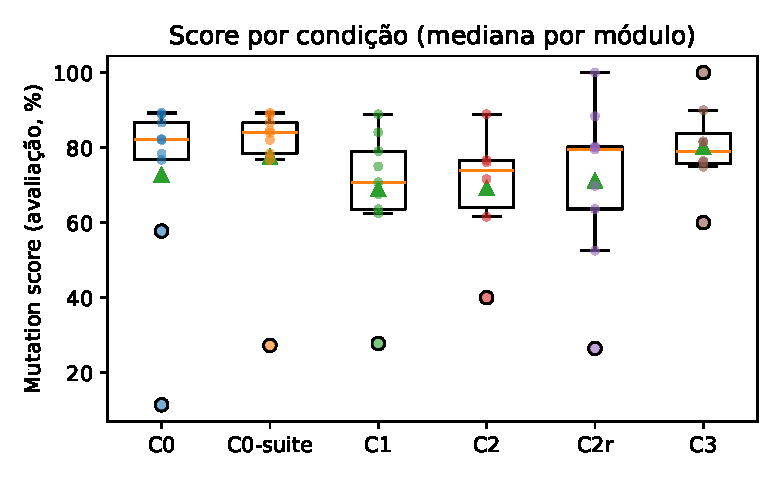
\includegraphics[width=0.78\linewidth]{figs/fig_ms_by_condition.pdf}
\caption{\textit{Mutation score} no grupo de avaliação por condição (um ponto por módulo, mediana das repetições; losango verde:
triângulo verde: média; pontos circulados: valores atípicos).}
\label{fig:ms}
\end{figure}

\textbf{H1 (não sustentada).} A mediana de \textit{score} no grupo de avaliação é 80,3\% em C3, contra 70,0\% em C1, 76,1\% em
C2 e 79,0\% em C2r (Tabela~\ref{tab:cond}). Só a comparação com C2 é significativa depois da correção de Holm (diferença
mediana de 12,2 pontos percentuais, IC 95\% [5,1; 17,4], $p_{\text{Holm}}=0{,}047$, $n=6$ módulos). Contra C1 (7,6 pp,
$p_{\text{Holm}}=0{,}109$, $n=8$) e contra C2r (4,0 pp, $p_{\text{Holm}}=0{,}109$, $n=8$) a diferença é positiva, mas os
intervalos incluem zero. Como H1 exige C3 $>$ C2r, e C2r é a comparação com orçamento igualado, não a consideramos
sustentada. Parte da vantagem de C3 sobre C1 e C2 é, portanto, compatível com o efeito de gastar mais chamadas: C2r e C3
consomem cerca de 10 vezes mais tokens que C1 e C2 (medianas de 52 mil e 64 mil contra 5,3 mil e 5,9 mil). Na análise de
sensibilidade, em que \textit{runs} sem teste válido contam como zero, o padrão se mantém (C3 $>$ C2 com $p_{\text{Holm}}=0{,}012$;
C3 $>$ C2r com $p_{\text{Holm}}=0{,}156$).

\textbf{Validade dos testes gerados.} A Tabela~\ref{tab:valid} mostra quanto do que o modelo gera é aproveitável.
\pendente{executar as condições com LLM para reportar a validade dos testes gerados}


\begin{table}[t]
\centering\small
\begin{tabular}{lrrrrr}
\toprule
Cond. & Runs & Runs v\'alidos & Taxa de runs (\%) & Itera\c{c}\~oes v\'alidas/tentadas & Taxa de itera\c{c}\~oes (\%) \\
\midrule
C1 & 27 & 23 & 85.2 & 23/27 & 85.2 \\
C2 & 27 & 17 & 63.0 & 17/27 & 63.0 \\
C2r & 27 & 24 & 88.9 & 113/162 & 69.8 \\
C3 & 27 & 23 & 85.2 & 105/162 & 64.8 \\
\bottomrule
\end{tabular}

\caption{Validade dos testes gerados por condição. ``Runs válidos'': ao menos uma iteração aprovada nos guardrails e no código original.
Falhas de infraestrutura (cota, \textit{timeout}) não são contadas.}
\label{tab:valid}
\end{table}

\textbf{Por que os testes são inválidos.} Em uma inspeção manual dos \textit{runs} de C2 sem teste válido
(\texttt{knitwork/string}, \texttt{ufo/url} e \texttt{ufo/utils}), todos terminaram com a mesma causa, testes que
falham no código original após os dois reparos (G3), e não por limite de cota ou \textit{timeout}. As falhas são
expectativas incorretas sobre o comportamento do código: por exemplo, o modelo supôs que \texttt{isAbsolute} devolve
\texttt{true} quando o código devolve um valor numérico, que \texttt{href} termina em barra quando não termina, ou
confundiu o escape de quebra de linha. Os reparos nem sempre ajudam: em um caso o modelo alterou a asserção errada e deixou a
falha original. Como o código atual é o oráculo, essas falhas indicam que o modelo erra o que o código faz, e não que o teste
seja inadequado.

\textbf{H2 (não sustentada).} Em C3, o ganho de cobertura de linha entre $k=0$ e $k=5$ é pequeno (mediana de 1,1 pp), porque a
cobertura já parte de valores altos (a mediana de C0 é 95,5\% e a de todas as condições com LLM, 100\%), enquanto o ganho de
\textit{score} no grupo de avaliação tem mediana de 9,8 pp ($n=6$ módulos). Portanto a premissa de que a cobertura sobe sem que o
\textit{score} suba na mesma proporção não se verifica (Figura~\ref{fig:h2}; $\Delta\text{cob}>\Delta\text{MS}$: $p=0{,}98$; Spearman entre os dois ganhos
$\rho=-0{,}15$, $p=0{,}77$; ambos com $p_{\text{Holm}}=1{,}00$). A lacuna entre cobertura e \textit{score} (cob.\ de linha $-$ MS\textsubscript{all}) é maior em C1 que no
\textit{baseline} humano (26,0 contra 19,5 pp; diferença mediana de 12,6 pp, $p_{\text{Holm}}=0{,}047$, $n=9$), isto é, testes
\textit{zero-shot} cobrem mais do que detectam. Em C3 a lacuna cai para 16,7 pp e fica próxima da humana (C3 contra C0, 2,3 pp,
$p_{\text{Holm}}=1{,}00$, $n=8$); a redução em relação a C2 ($-$9,2 pp, $n=6$) tem $p=0{,}031$ antes da correção, mas
$p_{\text{Holm}}=0{,}156$ depois, e portanto não é confirmada. Aplicamos Holm sobre os seis testes da família H2 (os dois de
ganhos e os quatro de lacuna). O critério de H2 (lacuna positiva que não diminui) não é atendido de forma consistente.

\begin{figure}[t]
\centering
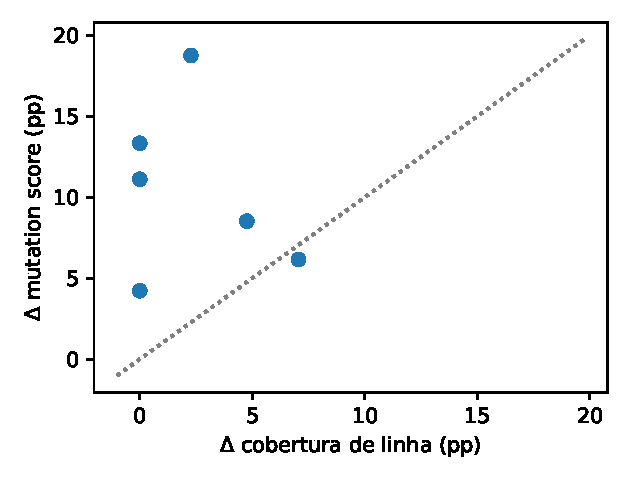
\includegraphics[width=0.62\linewidth]{figs/fig_h2_deltas.pdf}
\caption{H2: ganho de cobertura de linha e de \textit{mutation score} (grupo de avaliação) entre $k=0$ e $k=5$ em C3, por módulo
($n=6$). A diagonal marca ganhos iguais; cinco dos seis módulos ficam acima dela (o \textit{score} ganha mais que a
cobertura) e um fica abaixo.}
\label{fig:h2}
\end{figure}

\textbf{H3 (indício descritivo, sem significância).} A mediana do melhor \textit{score} até a iteração $k$ em C3 vai de 73,5\% em $k=0$
a 77,3\% em $k=1$ e a 78,9\% em $k=5$: a maior parte do ganho vem da primeira iteração, e as seguintes acrescentam pouco. O
custo por ponto percentual ganho cresce (mediana de cerca de 1,3 mil tokens por pp em $k=1$ para cerca de 4,8 mil em $k=5$), o
que é coerente com retorno decrescente. Os testes, porém, não rejeitam a hipótese nula (Friedman, $p=0{,}28$; tendência de Page,
$p=0{,}066$). As medianas por $k$ usam números diferentes de módulos (6 em $k=0$ e 8 em $k=5$, porque alguns módulos não tiveram
teste válido na geração inicial), então a curva é descritiva (Figura~\ref{fig:curva}). Na curva, a mediana por módulo de C2r
fica acima da de C3 em todas as iterações, inclusive em $k=5$ (79,5\% contra 78,9\%), o que difere da Tabela~\ref{tab:cond}
(80,3\% contra 79,0\%) porque as duas agregam de modos diferentes: a tabela usa a mediana dos \textit{runs} e a figura, a mediana
dos módulos que tiveram teste válido em cada $k$. As faixas interquartis se sobrepõem em grande parte, de modo que as duas
condições não se distinguem nesta amostra.

\begin{figure}[t]
\centering
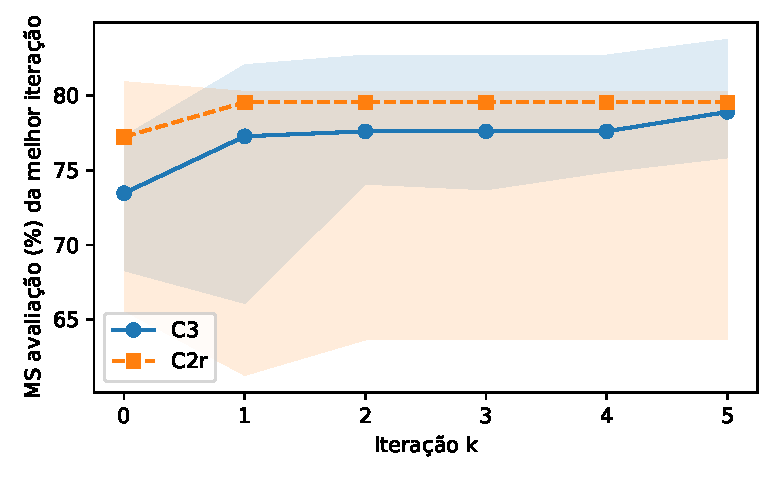
\includegraphics[width=0.78\linewidth]{figs/fig_curve_k.pdf}
\caption{Mediana por módulo do melhor \textit{mutation score} de avaliação até a iteração $k$, em C3 e C2r (faixa: intervalo
interquartil).}
\label{fig:curva}
\end{figure}

\subsection{Análises de sensibilidade}

\textbf{V1: memorização.} O \textit{probe} de memorização (\texttt{gemini-3.5-flash-lite}) foi executado antes de qualquer
\textit{run} de C1--C3, e o corte entre os estratos é a mediana da similaridade (0,141). Ficaram em baixa memorização
\texttt{defu}, \texttt{pathe/\_path}, \texttt{pathe/utils}, \texttt{ufo/punycode} e \texttt{ufo/url} (5 módulos), e em alta
\texttt{knitwork/string}, \texttt{ufo/parse}, \texttt{ufo/query} e \texttt{ufo/utils} (4 módulos). Com tão poucos módulos por
estrato, quase nenhum teste de H1 pode ser executado (exigimos ao menos 5 pares): na baixa memorização, C3 $>$ C1 e C3 $>$ C2r
(ambos com $n=5$) não são significativos ($p_{\text{Holm}}=0{,}44$), e na alta nenhuma comparação tem pares suficientes. A
Tabela~\ref{tab:v1} traz as medianas, que são só descritivas. Em baixa memorização C3 e C2r empatam (79,0\%); em alta, C3 fica
3,5 pontos percentuais acima de C2r, mas com $n$ de 3 a 4 módulos. C2 chega a 83,9\% na alta memorização, mas com só 6 de 12
\textit{runs} válidos, o que é o viés de sobrevivência descrito acima. Não há, portanto, evidência de que a memorização altere as conclusões, nem de que
não altere.

\begin{table}[t]
\centering\small
\begin{tabular}{lrrrr}
\toprule
 & \multicolumn{2}{c}{Baixa (5 módulos)} & \multicolumn{2}{c}{Alta (4 módulos)} \\
Cond. & $n$ & MS\textsubscript{eval} & $n$ & MS\textsubscript{eval} \\
\midrule
C0 & 5 & 82,1 & 4 & 70,0 \\
C1 & 12 & 71,7 & 11 & 69,7 \\
C2 & 11 & 63,6 & 6 & 83,9 \\
C2r & 14 & 79,0 & 10 & 78,2 \\
C3 & 14 & 79,0 & 9 & 81,7 \\
\bottomrule
\end{tabular}
\caption{V1: mediana do \textit{score} de avaliação por estrato de memorização ($n$: \textit{runs} válidos; C0: módulos).}
\label{tab:v1}
\end{table}

\textbf{V2: mutantes equivalentes.} Repetimos H1 sobre MS\textsubscript{killable}, o número de mutantes mortos dividido pela
união dos mortos por qualquer condição no módulo. Com essa métrica, C3 supera as três outras condições
(C3 $>$ C1: 9,8 pp, $p_{\text{Holm}}=0{,}047$, $n=8$; C3 $>$ C2: 12,7 pp, $p_{\text{Holm}}=0{,}047$, $n=6$; C3 $>$ C2r: 5,3 pp, IC 95\% [0,3; 10,6],
$p_{\text{Holm}}=0{,}047$, $n=8$). \textbf{Não tomamos isso como suporte a H1.} MS\textsubscript{killable} é calculado sobre todos os
mutantes, inclusive os do grupo de feedback que C3 otimiza e que C2r usa para escolher sua melhor amostra. Ela mistura exatamente
o sinal que o \textit{split} existe para separar, e por construção favorece C3. A métrica de H1 permanece o \textit{score} no grupo de
avaliação, em que C3 $>$ C2r não é significativo.

\textbf{V4: \textit{runs} instáveis.} Nenhum dos 129 \textit{runs} teve reexecução com resultado diferente (G6), então incluir ou excluir
\textit{runs} instáveis não altera nenhum resultado.

\textbf{V3: operadores.} O Stryker já foi usado com todos os operadores padrão, então não havia um segundo conjunto pronto. Definimos
um conjunto próprio, sobre a AST do TypeScript, com operadores que o Stryker não implementa: literal numérico $n\to n\pm1$, \texttt{return
expr} $\to$ \texttt{return undefined} e troca dos dois primeiros argumentos de uma chamada. Os mutantes são injetados por um
\textit{plugin} do Vite, sem alterar o código dos sujeitos, e cada teste final selecionado (e o teste humano de C0) foi reavaliado contra
eles (105 \textit{runs}; nenhum falhou no teste-base e nenhum mutante foi inválido). Como esses mutantes não participam do \textit{split}, não
há o viés visto na V2. A mediana do \textit{score} nesse conjunto foi 85,5 em C3, 83,5 em C2r, 80,0 em C2, 76,4 em C1 e 78,6 em C0, a mesma
ordenação do Stryker. Repetida sobre esse \textit{score}, H1 não é sustentada: C3 $>$ C1 ($p=0{,}063$, $p_{\text{Holm}}=0{,}188$, $n=8$),
C3 $>$ C2 ($p=0{,}125$, $p_{\text{Holm}}=0{,}188$, $n=6$) e C3 $>$ C2r ($p=0{,}094$, $p_{\text{Holm}}=0{,}188$, $n=8$; diferença mediana de 2,0 pp).
Ressalvas: o conjunto foi definido por nós, não é uma ferramenta independente, e alguns módulos geram poucos mutantes (cerca de 10 em
\texttt{defu} e \texttt{ufo/query}), o que produz empates. A V3 indica que o resultado não depende só dos operadores do Stryker, mas não
elimina o risco de \textit{overfitting} a mutantes sintéticos (ver a seção de ameaças).

\section{Discussão e ameaças à validade}
\label{sec:ameacas}

\textbf{Validade de construto.} O \textit{mutation score} subestima a qualidade quando há mutantes equivalentes; por isso
reportamos também $\text{MS}_{\text{killable}}$. Mutantes sintéticos não são defeitos reais, embora haja evidência de
correlação \cite{just2014}. Usamos o código atual como oráculo: um teste gerado que afirma um comportamento incorreto
mas atual passa e ``mata'' mutantes; não medimos corretude semântica das expectativas.

\textbf{Validade interna.} A estocasticidade do modelo é tratada com repetições e testes não paramétricos; o desvio de
modelos gratuitos, com ID fixo e janela de coleta curta; o \textit{overfitting} ao Stryker, com o \textit{split} (mitigação
parcial, pois a ferramenta é a mesma nos dois grupos; a reavaliação com um segundo conjunto de operadores, próprio e não independente, é a V3); e a comparação
injusta entre C1/C2 e C3, com C2r. Ainda assim C1 e C2 usam menos orçamento por construção.

\textbf{Viés de sobrevivência.} Runs em que nenhum teste gerado é válido não têm \textit{score} e saem da análise principal,
o que pode favorecer a condição que mais falha em módulos difíceis. Mitigamos reportando a taxa de validade por condição e
uma análise de sensibilidade em que esses \textit{runs} contam como \textit{score} zero, uma convenção conservadora (um conjunto
de testes que falha no código original equivale, na prática, a não ter testes) que não é a única possível; ela foi definida
depois de observadas as primeiras execuções.

\textbf{Validade externa.} Nove módulos de quatro bibliotecas de funções puras em TypeScript, de um mesmo ecossistema e com
um único modelo, não generalizam para código com estado, I/O ou outras linguagens.

\textbf{Memorização.} Bibliotecas populares provavelmente fazem parte do treino do modelo \cite{carlini2021}. Mitigamos com um
\textit{probe} que mede quanto da segunda metade do teste humano o modelo reproduz a partir da primeira, e estratificamos as
análises em baixa e alta memorização.

\textbf{Custo e governança.} O teste de mutação multiplica a execução da suíte; medimos de 23 s a 158 s por rodada em
1 vCPU, e uma coleta completa exige centenas de rodadas. O tier gratuito pode usar dados para treino (código aberto, risco
baixo) e impõe limites que podem forçar a coleta em vários dias. Há risco de alucinação de APIs e de testes frágeis; os
guardrails e a exigência de que os testes passem no código original mitigam, sem eliminar.

\section{Conclusão}

Apresentamos uma malha de \textit{continuous evals} guiada por mutação para geração de testes com LLM, com controle de
orçamento, \textit{hold-out} de mutantes, guardrails, protocolo estatístico e \textit{baseline} humano medido em 9 módulos reais. O
arcabouço está implementado, testado e validado de ponta a ponta, e a primeira execução das condições com LLM (um modelo,
9 módulos, 3 repetições) não sustenta H1: o laço de feedback supera C1 e C2, mas não se distingue da amostragem independente
com o mesmo orçamento (C2r). Também não sustenta H2 (a cobertura já parte de valores altos e o \textit{score} ganha mais que ela; a redução da lacuna
entre os dois com o laço não resiste à correção de Holm) e só dá
indícios descritivos de retorno decrescente (H3). A principal limitação é o poder: com 6 a 8 módulos pareados por comparação,
e com testes inválidos em até 37\% dos \textit{runs} de C2, diferenças pequenas não podem ser confirmadas nem descartadas.
Trabalhos futuros incluem uma revisão sistemática, mais bibliotecas e linguagens,
mais de um modelo, tratamento de mutantes equivalentes e avaliação com defeitos reais.

\bibliographystyle{apalike}
\bibliography{refs}

\end{document}
